\section{Frictionless SQL storage}
\begin{frame}[fragile]
  \frametitle{Frictionless SQL storage}
  \framesubtitle{\texttt{Pandas} Dataframe}
    \lstset{tabsize=2, language={Python}, basicstyle=\normalsize\ttfamily,
      keywordstyle=\color{blue}, rulesepcolor=\color{black},
      captionpos=bi, breaklines=true, escapechar=*, upquote=true,
      commentstyle=\color{green}\ttfamily, emph={requests, get, json, params},
      emphstyle={\color{red}}}
    \begin{lstlisting}
import pandas as pd
*\ldots * 
url = 'https://atlas.ripe.net/api/v1/probe'
res = get_json_from_url(url)
df = pd.DataFrame(res['objects'])
df.head()
    \end{lstlisting}
    \centering
    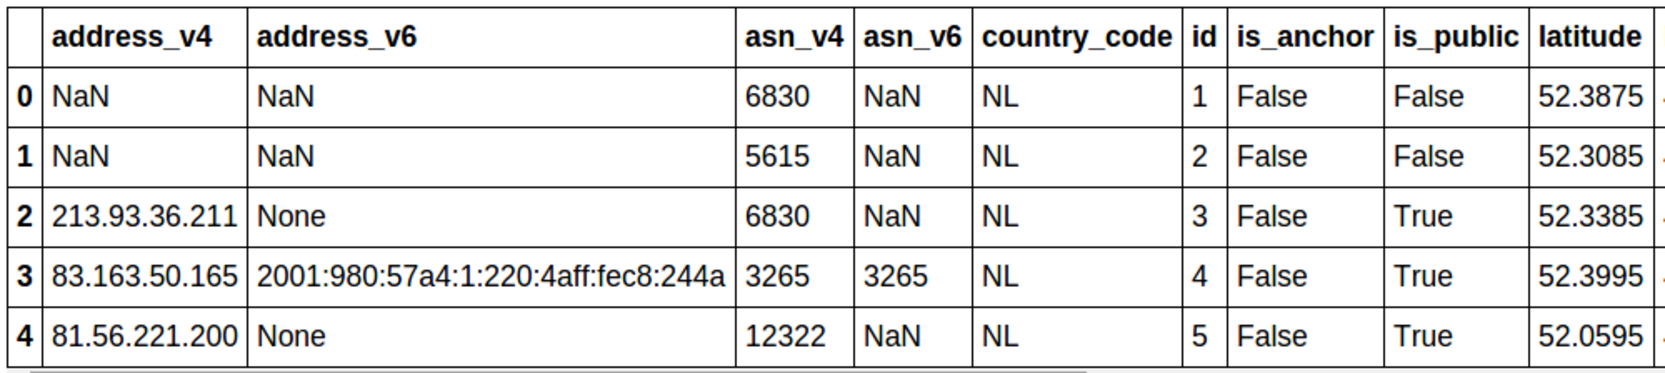
\includegraphics[width=1.0\linewidth]{figures/pandas-to-sql}\\
\end{frame}




\begin{frame}[fragile]
  \frametitle{Frictionless SQL storage}
  \framesubtitle{\texttt{import pandas as pd;} \texttt{pd.to\_sql(\dots)}}
    \lstset{tabsize=2, language={Python}, basicstyle=\normalsize\ttfamily,
      keywordstyle=\color{blue}, rulesepcolor=\color{black},
      captionpos=bi, breaklines=true, escapechar=*, upquote=true,
      commentstyle=\color{green}\ttfamily, emph={requests, get, json, params},
      emphstyle={\color{red}}}

    \begin{lstlisting}
import sqlite3
con = sqlite3.connect('$DB_LOCATION')
df.to_sql('$TABLENAME'
          , con
          , flavor='sqlite'
          , if_exists = 'append'
          , index_label = 'id'
         )
    \end{lstlisting}
\end{frame}

